Nous avons aussi modélisé le cycle de vie des unités à l'aide de deux diagrammes.

Le premier, un diagramme d'états-transitions \ref{fig:CycleVieUnite} nous permet de visualiser les différents cas posisbles lors du déplacement d'une unité et les différentes possibilités qui en découlent.
\begin{figure}[!h]
\centering
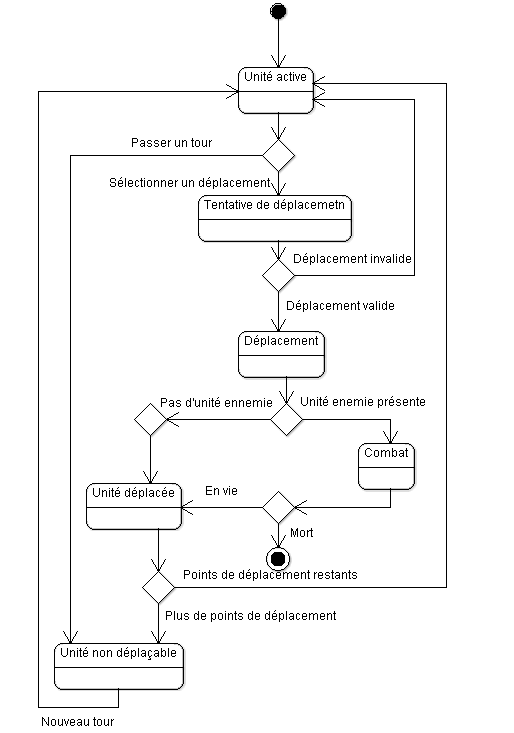
\includegraphics[width=\textwidth]{Parties/Images/CycleVieUnite.png}
\caption{Diagramme d'états-transitions : cycle de vie d'une unité}
\label{fig:CycleVieUnite}
\end{figure}

\bigbreak
Ensuite nous avons créé un diagramme de séquence \ref{fig:seq_DeplacementUnite} afin d'illustrer les traitements effectués par le jeu lorsque le joueur déplace une unité, c'est à dire la vérification de la validité du mouvement, et s'il est réalisable son éxécution ainsi que la résolution du combat si une unité adversaire est présente sur la case de destination.
\begin{figure}[!h]
\centering
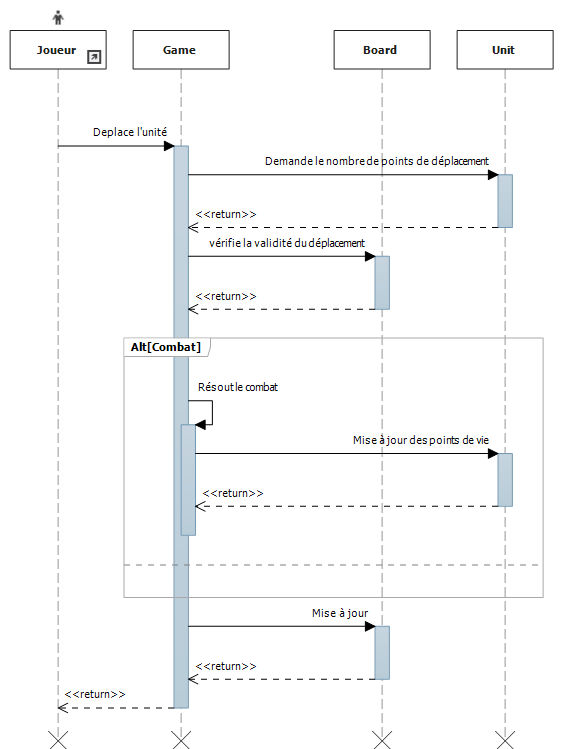
\includegraphics[width=\textwidth]{Parties/Images/seq_DeplacementUnite.png}
\caption{Diagramme de séquence : déplacement d'une unité}
\label{fig:seq_DeplacementUnite}
\end{figure}
